\section{Design}
\label{sec:Design}

\subsection{Architecture Design}
Because we selected the web application model from the beginning, we quickly decided to adopt the classic client-server architecture, which is a distributed application structure that partitions tasks or workloads between the providers of a resource or service, called servers, and service requesters, called clients. In theory, any device connected to the Internet can try to access and obtain the resources or services of the server while the server is running normally. Figure \ref{Client-Server Architecture} shows how it works.

\begin{figure}[htb]
\centering
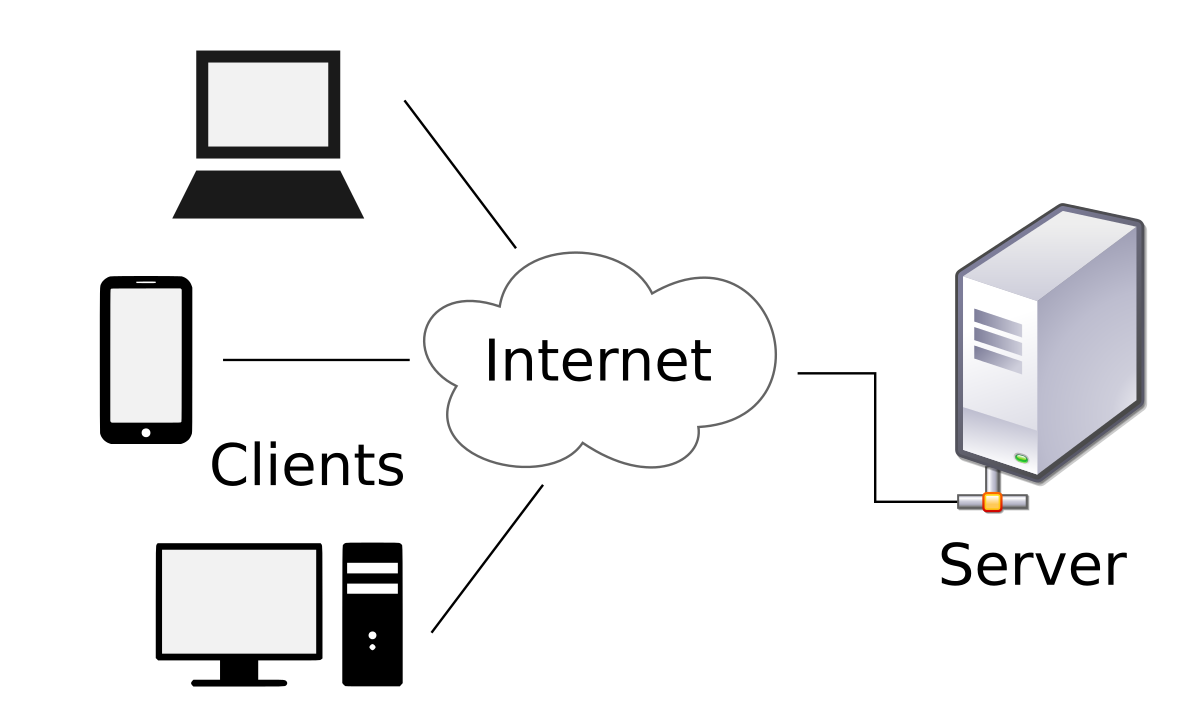
\includegraphics[width=\textwidth]{section03/assets/client_server.png}
\caption[the Architecture of Client-Server Model]{\label{Client-Server Architecture}the Architecture of Client-Server Model}
\end{figure}

Based on the client-server structure, we have detailed its component structures below:
\subsubsection{Web Browser or Client}
The web browser or client is the interface rendition of a web app functionality, with which the user interacts with. This content delivered to the client can be developed using HTML, JavaScript, and CSS and doesn’t require operating system related adaptations. In essence, the web browser or client manages how end users interact with the application.

There are three, well-known Web Application Architecture types available in the modern tech landscape: Single Page Applications (SPA), Microservices, and Serverless Architectures. Combine the actual situation and needs of this project, we chose the SPA.

\subsubsection{Web Application Server}
The web application server manages business logic and data persistence and can be built using PHP, Python, Java, Ruby, .NET, Node.js, among other languages. It’s comprised of at least a centralized hub or control center to support multi-layer applications.

\subsubsection{Database Server}
The database server provides and stores relevant data for the application. Additionally, it may also supply the business logic and other information that is managed by the web application server.

\subsection{Database Design}
This subsection gives a great deal of precise description supporting point 1.

\subsection{REST API Design}
\begin{table}[ht]
  \centering
  \begin{tabularx}{\textwidth}{>{\raggedright}cXX} % way of defining a fix columns width
    \toprule[1.5pt]
    \textit{HTTP Verb} & \textit{URI} & \textit{Description} \\
    \midrule[1.5pt]
    POST & /metro/auth/signup & Sign up for a new account \\
    \midrule
    POST & /metro/auth/login & Log in to the system \\
    \midrule
    POST & /metro/auth/logout & Log out of the system \\
    \midrule
    GET & /metro/api/v1/users & Get a list of all users \\
    \midrule
    GET & /metro/api/v1/users/\{id\} & Get the user with \{id\} \\
    \midrule
    GET & /metro/api/v1/users/\{uid\}/ maps & Get a list of all maps of the user with \{uid\} \\
    \midrule
    PATCH & /metro/api/v1/users/\{id\}/ password & Verify the password of the user with \{id\} \\
    \midrule
    PUT & /metro/api/v1/users/\{id\}/ password & Update the password of the user with \{id\} \\
    \midrule
    PUT & /metro/api/v1/users/\{id\}/ email & Update the email of the user with \{id\} \\
    \midrule
    PUT & /metro/api/v1/users/\{id\}/ name & Update the name of the user with \{id\} \\
    \midrule
    PUT & /metro/api/v1/users/\{id\}/ enabled & Update the enabled of the user with \{id\} \\
    \midrule
    GET & /metro/api/v1/maps/\{id\} & Get the map with \{id\} \\
    \midrule
    GET & /metro/api/v1/maps/ ?page=\{page\}\&limit=\{limit\} & Get a list of \{limit\} maps on page \{page\} \\
    \midrule
    POST & /metro/api/v1/maps & Add a new map to the database \\
    \midrule
    PUT & /metro/api/v1/maps/\{id\} & Update the map with \{id\} \\
    \midrule
    DELETE & /metro/api/v1/maps/\{id\} & Delete the map with \{id\} \\
    \bottomrule[1.5pt]
  \end{tabularx}
  \caption[REST API Design Table]{REST API Design Table}
  \label{REST API Design Table}
\end{table}

\subsection{Map Generator Design}
